%input macros (i.e. write your own macros file called MacroFile1.tex)
%\newcommand{\PdfPsText}[2]{
  \ifpdf
     #1
  \else
     #2
  \fi
}

\newcommand{\IncludeGraphicsH}[3]{
  \PdfPsText{\includegraphics[height=#2]{#1}}{\includegraphics[bb = #3, height=#2]{#1}}
}

\newcommand{\IncludeGraphicsW}[3]{
  \PdfPsText{\includegraphics[width=#2]{#1}}{\includegraphics[bb = #3, width=#2]{#1}}
}

\newcommand{\InsertFig}[3]{
  \begin{figure}[!htbp]
    \begin{center}
      \leavevmode
      #1
      \caption{#2}
      \label{#3}
    \end{center}
  \end{figure}
}


%%% Local Variables: 
%%% mode: latex
%%% TeX-master: "~/Documents/LaTeX/CUEDThesisPSnPDF/thesis"
%%% End: 


 \documentclass[oneside,12pt]{Classes/CUEDthesisPSnPDF}


\ifpdf
    \pdfinfo { /Title  (CUED PhD and MPhil Thesis Classes)
               /Creator (TeX)
               /Producer (pdfTeX)
               /Author (PengFei Li u4959060@anu.edu.au)
               /CreationDate (D:20130527000000)  %format D:YYYYMMDDhhmmss
               /ModDate (D:20030815213532)
               /Subject (Algorithms for Meta-Search)
               /Keywords (Honours, Thesis)}
    \pdfcatalog { /PageMode (/UseOutlines)
                  /OpenAction (fitbh)  }
\fi

\title{Algorithms for Metasearch\\[1ex]}

\ifpdf
  \author{\href{mailto:u4959060@anu.edu.au}{Peng-Fei Li}}
  \collegeordept{\href{http://cecs.anu.edu.au}{College of Engineering and Computer Science
}}
  \university{\href{http://www.anu.edu.au}{The Australian National University}}
% insert below the file name that contains the crest in-place of 'UnivShield'
  \crest{
\includegraphics[width=30mm]{UnivShield}}
\else
  \author{Peng-Fei Li}
  \collegeordept{College of Engineering and Computer Science}
  \university{The Australian National University}
% insert below the file name that contains the crest in-place of 'UnivShield'
  \crest{
\includegraphics[bb = 0 0 292 336, width=50mm]{UnivShield}}
\fi
%
% insert below the file name that contains the crest in-place of 'UnivShield'
% \crest{\IncludeGraphicsW{anu_logo.jpg}{40mm}{14 14 73 81}}
%
%\renewcommand{\submittedtext}{change the default text here if needed}
\degree{Honors}
\degreedate{}

% turn of those nasty overfull and underfull hboxes
\hbadness=10000
\hfuzz=50pt

% Put all the style files you want in the directory StyleFiles and usepackage like this:
\usepackage{StyleFiles/watermark}

% Comment out the next line to get single spacing
\onehalfspacing

\begin{document}

%\language{english}

% A page with the abstract on including title and author etc may be
% required to be handed in separately. If this is not so, then comment
% the below 3 lines (between '\begin{abstractseparte}' and 
% 'end{abstractseparate}'), normally like a declaration ... needs some more
% work, mind as environment abstracts creates a new page!
% \begin{abstractseparate}
%   \chapter*{Abstract}  % the * means don't put a number in the title
\addcontentsline{toc}{chapter}{Abstract} % but add it to the table of contents

Result merging problems have been a significant issues in federated search. However, there exist no general algorithms that can work well in all situations and no particular algorithm can defeat another in every environment. In this paper, we examine several approaches that are widely used in this area. We built a meta-search engine based on the search engines that are distributed among different departments of The Australian National University. Several merging algorithms have been considered their feasibility to fit into the environment and some are implemented as the broker merging function. The algorithms are then be evaluation based on a manually judgement system and NDCG measurement is applied to compare their performance. The result shows that [to be continue]. And then we proposed a [to be continue] algorithm, and experiment shows that[to be continue].


% \end{abstractseparate}




% Using the watermark package which is in StyleFiles/
% and to remove DRAFT COPY ONLY appearing on the top of all pages comment out below line
%\watermark{DRAFT COPY ONLY}


\maketitle

%set the number of sectioning levels that get number and appear in the contents
\setcounter{secnumdepth}{3}
\setcounter{tocdepth}{3}

\frontmatter % book mode only
\pagenumbering{roman}
% Thesis Dedictation ---------------------------------------------------

\begin{dedication} %this creates the heading for the dedication page

I would like to dedicate this thesis to my loving parents ...

\end{dedication}

% ----------------------------------------------------------------------

%%% Local Variables: 
%%% mode: latex
%%% TeX-master: "../thesis"
%%% End: 

% Thesis Acknowledgements ------------------------------------------------


%\begin{acknowledgementslong} %uncommenting this line, gives a different acknowledgements heading
\begin{acknowledgements}      %this creates the heading for the acknowlegments


And I would like to acknowledge ...


\end{acknowledgements}
%\end{acknowledgmentslong}

% ------------------------------------------------------------------------

%%% Local Variables: 
%%% mode: latex
%%% TeX-master: "../thesis"
%%% End: 

\chapter*{Abstract}  % the * means don't put a number in the title
\addcontentsline{toc}{chapter}{Abstract} % but add it to the table of contents

Result merging problems have been a significant issues in federated search. However, there exist no general algorithms that can work well in all situations and no particular algorithm can defeat another in every environment. In this paper, we examine several approaches that are widely used in this area. We built a meta-search engine based on the search engines that are distributed among different departments of The Australian National University. Several merging algorithms have been considered their feasibility to fit into the environment and some are implemented as the broker merging function. The algorithms are then be evaluation based on a manually judgement system and NDCG measurement is applied to compare their performance. The result shows that [to be continue]. And then we proposed a [to be continue] algorithm, and experiment shows that[to be continue].



\tableofcontents
\listoffigures
\printnomenclature  %% Print the nomenclature
\addcontentsline{toc}{chapter}{Nomenclature}

\mainmatter % book mode only
%%% Thesis Introduction --------------------------------------------------
\chapter{Introduction}
\ifpdf
    \graphicspath{{Introduction/IntroductionFigs/PNG/}{Introduction/IntroductionFigs/PDF/}{Introduction/IntroductionFigs/}}
\else
    \graphicspath{{Introduction/IntroductionFigs/EPS/}{Introduction/IntroductionFigs/}}
\fi

And this is how I would like to introduce my piece of work ...


blah blah blah blah blah blah blah blah blah blah blah blah blah blah blah blah blah blah blah blah blah blah blah blah blah blah blah blah blah blah blah blah blah blah blah blah blah blah blah blah blah blah blah blah blah blah blah blah blah blah blah blah blah blah blah blah blah blah blah blah blah blah blah blah blah blah blah blah blah blah blah blah blah blah blah blah blah blah blah blah blah blah blah blah blah blah blah blah blah blah blah blah blah blah blah blah blah blah blah blah blah blah blah blah blah blah blah blah blah blah blah blah blah blah blah blah blah blah blah blah blah blah blah blah blah blah blah blah blah blah blah blah blah blah blah blah blah blah blah blah blah blah blah blah blah blah blah blah blah blah blah blah blah blah blah blah blah blah blah blah blah blah blah blah blah blah blah blah blah blah blah blah blah blah blah blah blah blah blah blah blah blah blah blah blah blah blah blah blah blah blah blah blah blah blah blah blah blah blah blah blah blah blah blah blah blah blah blah blah blah blah blah blah blah blah blah blah blah blah blah blah blah blah blah blah blah blah blah blah blah blah blah blah blah blah blah blah blah blah blah blah blah blah blah blah blah blah blah blah blah blah blah blah blah blah blah blah blah blah blah blah blah blah blah blah blah blah blah blah blah blah blah blah blah blah blah blah blah blah blah blah blah blah blah blah blah blah blah blah blah blah blah blah blah blah blah blah blah blah blah blah blah blah blah blah blah blah blah blah blah blah blah blah blah blah blah blah blah blah blah blah blah blah blah blah blah blah blah blah blah blah blah blah blah blah blah blah blah blah blah blah blah blah blah blah blah blah blah blah blah blah blah blah blah blah blah blah blah blah blah blah blah blah blah blah blah blah blah blah blah blah blah blah blah blah blah blah blah blah blah blah blah blah blah blah blah blah blah blah blah blah blah blah blah blah blah blah blah blah blah blah blah blah blah blah blah blah blah blah blah blah blah blah blah blah blah blah blah blah blah blah blah blah blah blah blah blah blah blah blah blah blah blah blah blah blah blah blah blah blah blah blah blah blah blah blah blah blah blah blah blah blah blah blah blah blah blah blah blah blah blah blah blah blah blah blah blah blah blah blah blah blah blah blah blah blah blah blah blah blah blah blah blah blah blah blah blah blah blah blah blah blah blah blah blah blah blah blah blah blah blah blah blah blah blah blah blah blah blah blah blah blah blah blah blah blah blah blah blah blah blah blah blah blah blah blah blah blah blah blah blah blah blah blah blah blah blah blah blah blah blah blah blah blah blah blah blah blah blah blah blah blah blah blah blah blah blah blah blah blah blah blah blah blah blah blah blah blah blah blah blah blah blah blah blah blah blah blah blah blah blah blah blah blah blah blah blah blah blah blah blah blah blah blah blah blah blah blah blah blah blah blah blah blah blah blah blah blah blah blah blah blah blah blah blah blah blah blah blah blah blah blah blah blah blah blah blah blah blah blah blah blah blah blah blah blah blah blah blah blah blah blah blah blah blah blah blah blah blah blah blah blah blah blah blah blah blah blah blah blah blah blah blah blah blah blah blah blah blah blah blah blah blah blah blah blah blah blah blah blah blah blah blah blah blah blah blah blah blah blah blah blah blah blah blah blah blah blah blah blah blah blah blah blah blah blah blah blah blah blah blah blah blah blah blah blah blah blah blah blah blah blah blah blah blah blah blah blah blah blah blah blah blah blah blah blah blah blah blah blah blah blah blah blah blah blah blah blah blah blah blah blah blah blah blah blah blah blah blah blah blah blah blah blah blah blah blah blah blah blah blah blah blah blah blah blah blah blah blah blah blah blah blah blah blah blah blah blah blah blah blah blah blah blah blah blah blah blah blah blah blah blah blah blah blah blah blah blah blah blah blah blah blah blah blah blah blah blah blah blah blah blah blah blah blah blah blah blah blah blah blah blah blah blah blah blah blah blah blah blah blah blah blah blah blah blah blah blah blah blah blah blah blah blah blah blah blah blah blah blah blah blah blah

%%% ----------------------------------------------------------------------


%%% Local Variables: 
%%% mode: latex
%%% TeX-master: "../thesis"
%%% End: 

% \pagebreak[4]
% \hspace*{1cm}
% \pagebreak[4]
% \hspace*{1cm}
% \pagebreak[4]

\chapter{My First Chapter But Note The Numbering ...}
\ifpdf
    \graphicspath{{Chapter1/Chapter1Figs/PNG/}{Chapter1/Chapter1Figs/PDF/}{Chapter1/Chapter1Figs/}}
\else
    \graphicspath{{Chapter1/Chapter1Figs/EPS/}{Chapter1/Chapter1Figs/}}
\fi

\section{First Paragraph}
And now I begin my first chapter here ...

Here is an equation\footnote{the notation is explained in the nomenclature section :-)}:
\begin{eqnarray}
CIF: \hspace*{5mm}F_0^j(a) &=& \frac{1}{2\pi \iota} \oint_{\gamma} \frac{F_0^j(z)}{z - a} dz
\end{eqnarray}
\nomenclature[zcif]{$CIF$}{Cauchy's Integral Formula}                                % first letter Z is for Acronyms 
\nomenclature[aF]{$F$}{complex function}                                                   % first letter A is for Roman symbols
\nomenclature[gp]{$\pi$}{ $\simeq 3.14\ldots$}                                             % first letter G is for Greek Symbols
\nomenclature[gi]{$\iota$}{unit imaginary number $\sqrt{-1}$}                      % first letter G is for Greek Symbols
\nomenclature[gg]{$\gamma$}{a simply closed curve on a complex plane}  % first letter G is for Greek Symbols
\nomenclature[xi]{$\oint_\gamma$}{integration around a curve $\gamma$} % first letter X is for Other Symbols
\nomenclature[rj]{$j$}{superscript index}                                                       % first letter R is for superscripts
\nomenclature[s0]{$0$}{subscript index}                                                        % first letter S is for subscripts

\section{Second Paragraph}
and here I write more ...\cite{texbook}

\subsection{sub first paragraph}
... and some more ...

Now I would like to cite the following: \cite{latex} and \cite{texbook}
and \cite{Rud73}.

I would also like to include a picture ...

\begin{figure}[!htbp]
  \begin{center}
    \leavevmode
    \ifpdf
      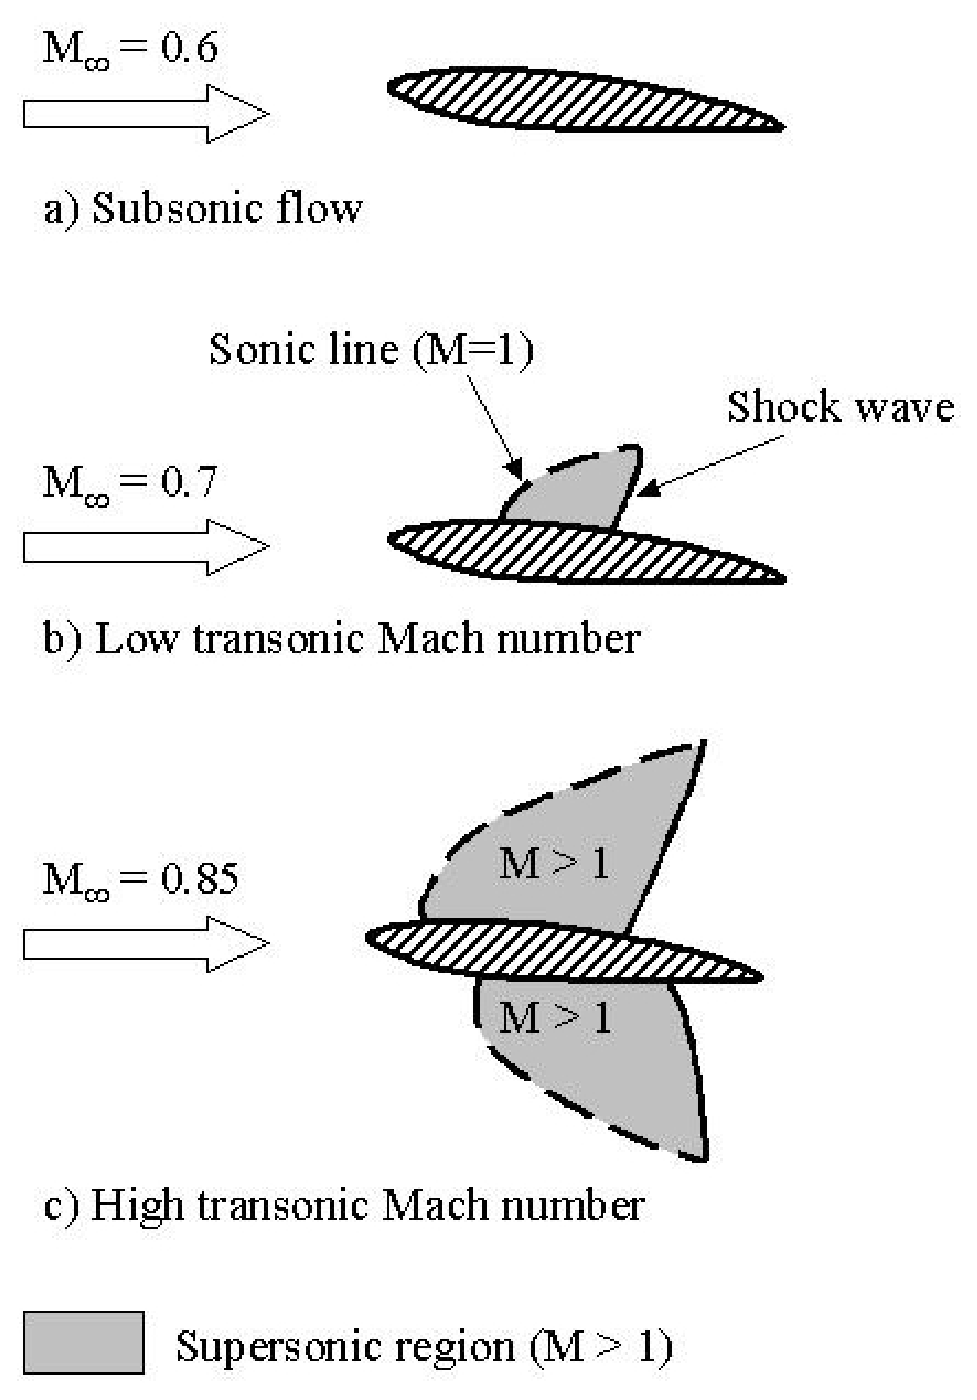
\includegraphics[height=6in]{aflow}
    \else
      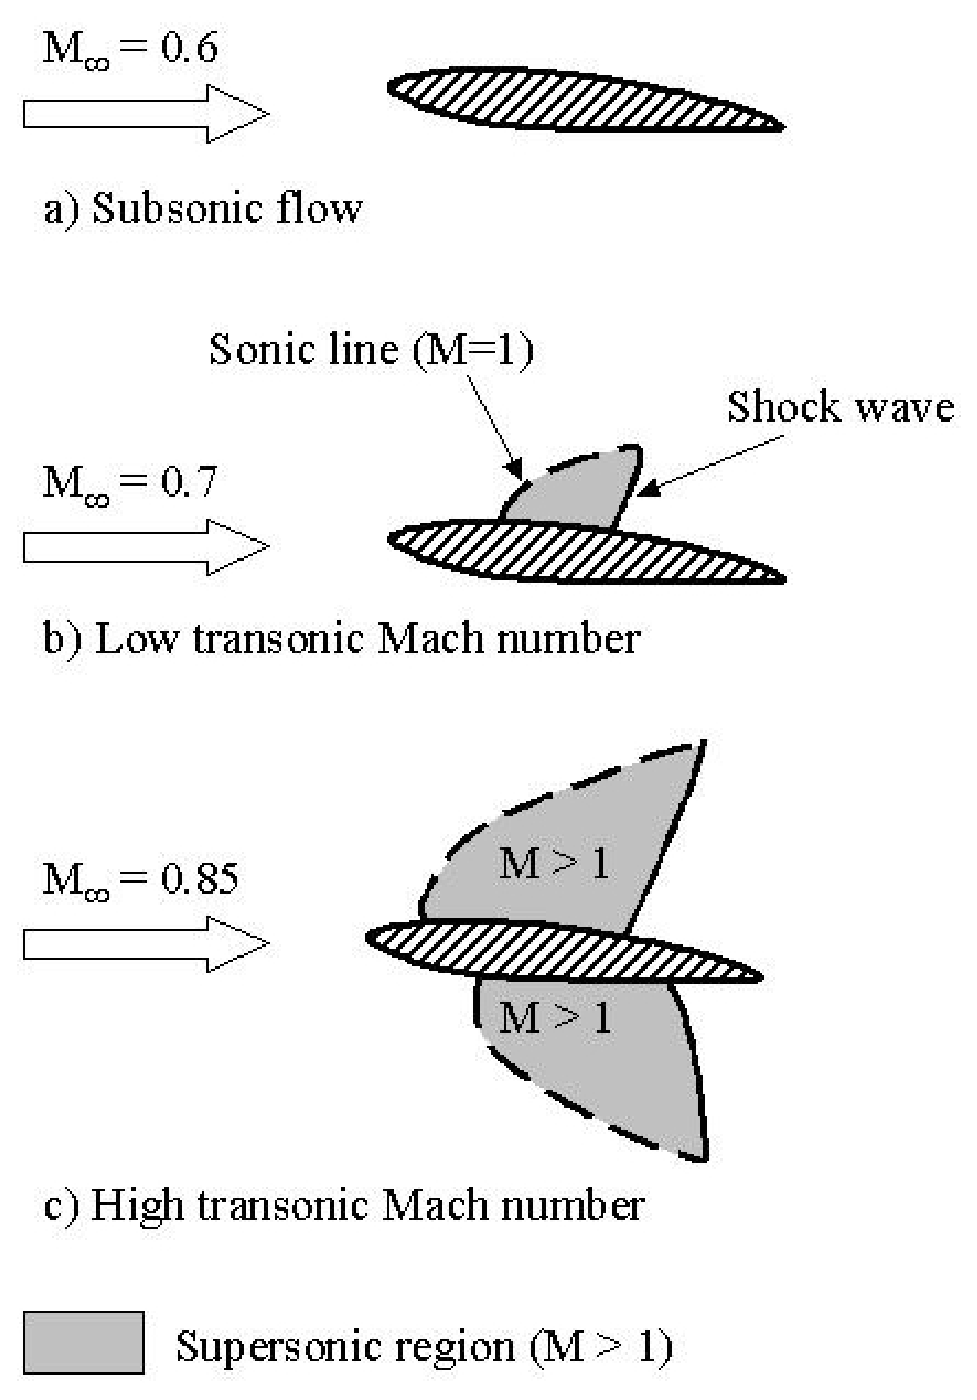
\includegraphics[bb = 92 86 545 742, height=6in]{aflow}
    \fi
    \caption{Airfoil Picture}
    \label{FigAir}
  \end{center}
\end{figure}

% above code has been macro-fied in Classes/MacroFile.tex file
%\InsertFig{\IncludeGraphicsH{aflow}{6in}{92 86 545 742}}{Airfoil Picture}{FigAir}

So as we have now labelled it we can reference it, like so (\ref{FigAir}) and it
is on Page \pageref{FigAir}. And as we can see, it is a very nice picture and we
can talk about it all we want and when we are tired we can move on to the next
chapter ...

I would also like to add an extra bookmark in acroread like so ...
\ifpdf
  \pdfbookmark[2]{bookmark text is here}{And this is what I want bookmarked}
\fi
% ------------------------------------------------------------------------


%%% Local Variables: 
%%% mode: latex
%%% TeX-master: "../thesis"
%%% End: 

\chapter{Literature Review}


The Internet has grown to be anocean with vast amount of data since its born. Discovering useful information among the massive amount of resources existing on the Internet has been a hot topic for years, which brought the rise of the field of information retrieval. Index centralised searching engines like Google is typical solution to this task. Traditional searching engines use crawlers or spiders to crawl information among the pages and then index the fetched pages. However, this procedure has a disadvantage due to its inability to retrieval information from Deep Web\cite{Bergman2001}. But as a matter of fact, most of the sites existing on the Internet nowadays are generated dynamically by fetching data from its background data, these data are deep hidden from the surface web that index centralised searching engines can analysis. The size of deep web is much larger than surface web, as pointed out by Bergman \cite{Bergman2001}, and is growing rapidly. 
\section{Meta-Search}
An alternative approach is to provide an integrated search engine that can send users' query to different search engines and then return the merged result. This method leaves the searching job to each component search engine, built into the document collection, which can retrieval its documents through its internal database. This approach is named distributed search\cite{Callan2000}, sometimes named federated search\cite{Jacso2004} or metasearch. A typical meta-search engine grabs users' query request, do some query expansion, which is optional, and then sends the query to different component search engines, finally the engine collection the results returned by all the collections and merging the resulting in a suitable ranking to display to users (Figure 2.1).
\begin{figure}[h!]
    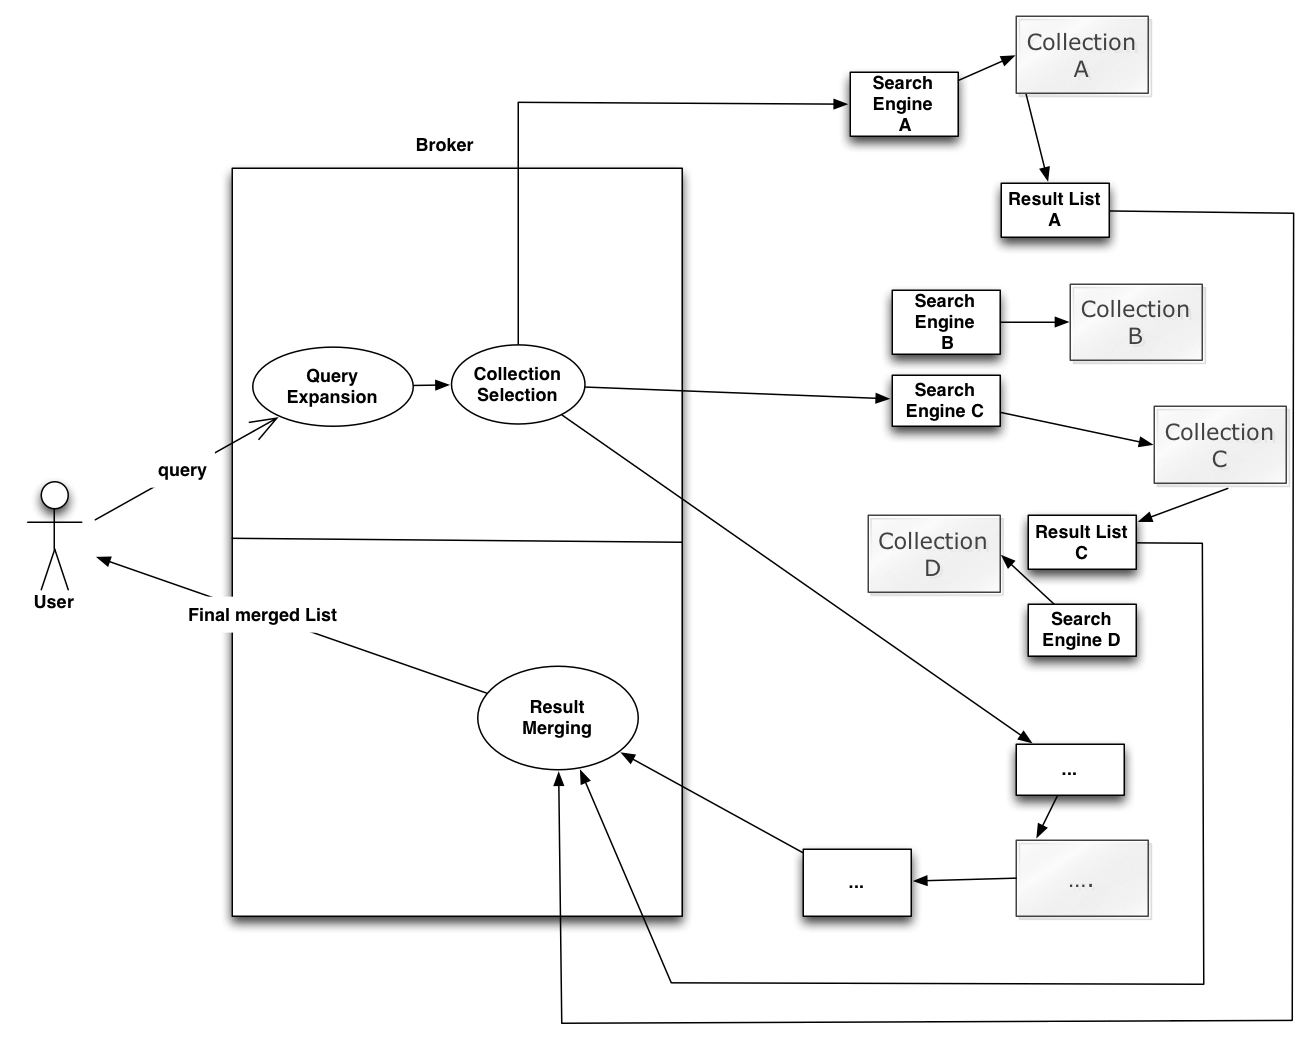
\includegraphics[width=12cm]{architecture.jpg}
\caption{A typical architecture of metasearch, the users' requests are fetched by the main component, which is named broker, some query expansion may be executed and the processed query will send to different collections. The collections execute searching on the query and return the retrieval results to the broker and then the }
\label{}
\end{figure}
\section{Collection Selection}
An efficiency issue may arise when the meta-search engine have to search across massive amount of collections. As a matter of fact, because some collection are mainly focused on a particular topic, many of the collections will contain limited number of documents that are relevant to the users' query, or even no documents will return in some extreme cases. Due to the limitation of memory, bandwidth, time and other resources, it would be a good idea to ignore some collections that are likely to be the last ones to have relevant documents with respect to a particular query or topic in semantic aspect. That problems has been defined as collection selection problems and have attracted many attentions by scientists in this area. Early meta-search engines apply manually cluster collections into different themes or topics and then assign query to different clusters according to its topic, it has already been tried to group collection automatically\cite{Danzig1991}. Later attempts have been made to treat each collection as a big document and then calculate the similarity between the collection and the query using the bag of words model. In this model, each collection is treated as a big document and other statistic information is stored for later use. A vector space model can be build using the big bag words model, in which all collections as well as queries are built into vectors. Each element into the vector represent the weight of a term to a collection or a query. The weight is often set by the TF-IDF weight which maybe obtained from the cooperative collection statistics or estimation and is used to calculate the similarity of documents or queries. Cosine similarity and Okapi BM25\cite{Robertson1994} are widely used to get the similarity of a collection and a query, which is also regard as the collection score in these algorithms. There are also many algorithms based on the lexicon information of the collection. For example, CORI\cite{Callan1995,Callan2000} is developed based on an information retrieval system named INQUERY\cite{Callan1992}, which builds an inference network to search information in a collection. The CORI system calculate the belief of a collection associated to a query and rank them according to the score. Besides all these lexicon based algorithms, document surrogate methods\cite{Si2003}\cite{Shokouhi2007}\cite{Thomas2009} and machine learning approaches \cite{Voorhees1995}have also come into use in this area.
\section{Result Merging}
Although collection is a significant issue in many systems and has drawn many attentions recent years, it is still a prior procedure of metasearch. It is quite important factor with related to the speed of the system as well as precision of the final result. However, in some cases when the number of collection is not very big, it may be a fact that the collection selection procedure may decrease the efficiency as well as precision since its incomplete searching. As the results are returned from different sub-components, it becomes another issue how to put them together into an integrated result list. Documents in these results lists are distributed differently and there is limited information about the result document in most cases. This problem has been defined as result merging or ranking fusion problems. A formal definition has been given to define ranking fusion problems by  \cite{Dwork2001} and \cite{Renda2003}. Given a set of items denoted by $U$, 	$\tau$ is an ordered list of the elements in a subset of $U$, which is denoted by $S$, for example, $\tau$=[$x_1$$\geq$$x_2$$\geq$$\cdotp$$\cdotp$$\cdotp$$\geq$$x_k$], where $x_i$$\in$$S$. If $\tau$ contains all the elements of $U$, $tau$ is said to be a $full list$ . However, full lists are not possible in most cases because the searching engines will not return all the items in the database as a limitation of resources. Assume a set of rank lists $R$=\{$\tau_1$,$\tau_2$,$\tau_3$,$\cdotp$$\cdotp$$\cdotp$,$\tau_n$\}, the result merging or rank fusion problem is to find out a new rank list, denoted by $\hat{\tau}$, which is the result of a rank fusion method applied to the rank lists in $R$.
\subsection{Round-Robin}
Previous meta-search merge the different lists into a unified one in a simple Round-Robin manner\cite{Rasolofo2003}. The round-robin algorithm is based on the assumption that the number of relevant documents is approximately the same and distributed evenly in all the collections\cite{Rasolofo2003}\cite{Rasolofo2001}. But the assumption cannot hold in a real world, where the number of relevant documents varies and the distribution is extraordinarily messy. Rasolofo et.al.\cite{Rasolofo2003}also proved that the round-robin method perform various randomly. It's may be a better idea to give weight to different collection to determine the order of collections when doing round-robin, which can make the method more stable. So they added some features to each collection to form a biased round-robin algorithm that different collections have collection scores showing their preference in each round-robin circle\cite{Rasolofo2003} and saw some precision increase.
\subsection{Score-based Methods}
It may be an advantage of knowing score information of each document in a collection, document score can be easily reused to get them into the right place into the universal list. Because document scores in different collections are always not comparable, a new score function should be generated to return comparable scores. Normalisation is approach used by many algorithms to generate the final score, for example, \cite{Renda2003} introduced two basic normalisation function, $Score normalisation$(euqation2.1) and $Z-score normalisation$(equation 2.2) .
\begin{equation}
w^{\tau}(i)=\frac{s^\tau(i)-min_{j\in\tau}s^\tau(j)}{max_{j\in\tau}s^\tau(j)-min_{j\in\tau}s^\tau(j)}
\end{equation}
$w^{\tau}(i)$ indicates the normalised weight of item $i\in\tau$, and the score of an item assigned by $\tau$ is denoted by $s^\tau(i)$
\begin{equation}
w^{\tau}(i)=\frac{s^\tau(i)-\mu_{s^\tau}}{\sigma_{s^\tau}}
\end{equation}
$\mu_{s^\tau}$ denotes the means of scores and $\sigma_{s^\tau}$ is the standard deviation.
In most cases, the score of each document is not available to meta-search systems. An alternative way is to estimate the score according to accessible information. \cite{Rasolofo2003} utilised various document fields to estimate the document score. They generate the document score using a generic document scoring function(Equation 2.3).
\begin{equation}
w_{ij}=\frac{NQW_i}{\sqrt{L_q^2+LF_i^2}}
\end{equation}
$NQW_i$  is the number of query words appearing in the processed field of the document i, $L_q$ is the length (number of words) of the query, and $LF_i$ is the length of the processed field of the document i. Then they use the score as the bases for their two new algorithms, namely SM-XX and RR-XX. The SM-XX algorithm use the estimated document score as the unified document score and merge all the documents in the order of the score. The other algorithm, use the score to re-rank the results in each collection and use the round-robin method to merge the new result lists. The "XX" stands for the document fields such as document title, document summary. Although it shows that the final result of RR-XX is better than original round-robin algorithm, it still leave the distribution of documents in each collection as a problem. 

Linear combination is another approach to get the final score of documents, for example, Fox and Shaw\cite{Fox1994a} developed 6 methods to normalise the overall similarity across all the individual searching systems based on SMART by combining the scores across all the collections. 
\begin{table}[ht]
\caption{Comb Algorithms} % title of Table
\centering % used for centering table
\begin{tabular}{l l } % centered columns (4 columns)
\hline\hline %inserts double horizontal lines
Name��� & Similarity�\\ [0.5ex] % inserts table
%heading
\hline % inserts single horizontal line
CombMAX & MAX(Individual Similarities)�������������������������������� \\ 
��������CombMIN & MIN(Individual Similarities)�������������������������������� \\ 
��������CombSUM & SUM(Individual Similarities)�������������������������������� \\ 
��������CombANZ & Number of Nonzero Similarities������������������������������ \\ 
��������CombMNZ & SUM(Individual Similarities)* Number of Nonzero Similarities \\ 
��������CombMED & MED(Individual Similarities)�������������������������������� \\ [1ex] % [1ex] adds vertical space
\hline %inserts single line
\end{tabular}
\label{table:nonlin} % is used to refer this table in the text
\end{table}
These 6 algorithms(Table 2.1), uses aggregation methods to estimate the location of a document among all the item sets. As discussed by the authors, is trying to eliminate the two types of primary errors in ranking methods, namely assigning a relatively high rank to a non-relevant document and assigning a relatively low rank to a relevant document. However, it's an obvious fact that both CombMIN and CombMAX combination method bring opposite effects. For CombMIN method, it can eliminate the possibility that a non-relevant document being assigned a high rank, however, the problem that CombMAX trying to fix has been amplified. The same effect exits when applying CombMIN method. And they also conduct some experiments all the combination algorithms and found that CombMNZ is the performs best among all the others. These score based algorithms can achieve great efficiency in precision and recall when the overlap between collection is very large and has been used as a baseline algorithm for many other papers. However, in real world application, the result returned by different collections are seldom having duplication, which means many of the documents will appear once in all the collections. The fact will bring very challenging difficulties to the combination methods. \cite{Vogt1998} also proposed a linear combination model named LC Model, which takes the weight of collection into consideration.

\subsection{Rank-based Methods}
Although in most cases, the score information of each document are not given in most scenarios, or cost too much complexity to estimate, ranking information of a document in a collection is presented in an obvious way, like is the order in the result list. Many algorithms are based on the ranking score of document, for example, Borda-fuse\cite{Aslam2001} was a voting procedure popularly used in Election scenario, and was modified to apply to our metasearch systems. In this model, servers are acting as the role of voter, and each document is just like the �candidate�. Each server or retrieval system holds its own preference of ranking on all the documents. And then, the top ranked documents are assigned c points for candidates whose size is c, and c-1 points for the next, etc. Then we sum the score of each document and rank them according to the score. Due to the facts that different server may have different weight on different topics, they assigned weights to each server and then modified the method to a weighted borda-fuse algorithm. This model, works quite well for the system, which has many overlap in the documents. However, in reality, the repositories may vary quite differently. In that case, each document may just appears once in each rank list, which means they may distributed evenly among all the searching systems and has a lot of documents with the same scores. So the model cannot work well in the situation when there is little intersection within documents. And as a fact, their experiments showed that the new algorithm cannot outperform the baseline algorithm, but in most case, can perform better than the best-input system. \cite{Renda2003} also proved that Borda-fuse algorithm is not competitive with score-based algorithms. 
\cite{Lee1997}\cite{Dwork2001} to be described...

\subsection{Collection weight}
It is a fact that different collection have a different weight on different queries or topics, for example, an electronic online shop is more likely to contain information about a PC than a bookshop website. The metasearch system should be a bias decider on different collection both on semantic relationship and  the volume of results they returned. Many of the previous algorithms have weighted versions. CORI\cite{Callan2000,Callan1995} uses a simple linear combination method to normalise the collection score(equation 2.4),
\begin{equation}
	C'=\frac{C-C_{min}}{C_{max}-C_{min}}
\end{equation} , the normalised score is then used by the raw score based function to estimate the document score by equation 2.5:
\begin{equation}
	D'=\frac{D+0.4\times{D}\times{C'}}{1.4}
\end{equation} 
Rasolofo et.al. \cite{Rasolofo2001}proposed a new approach to rank the list from different collections names LMS(using result Length to calculate Merging Score). They estimate the collection score by the The algorithm uses the result length, namely the number of documents retrieved by the collection using equation 2.6. $l_i$ is the number of documents returned by a collection and K is a constant set to 600. $C$ is the number of collections.
\begin{equation}
	S_i=\log{1+\frac{l_i\times{K}}{\sum\nolimits_{j=1}^{|C|}l_i}}
\end{equation}
The collection score was then used to generate a collection weight.
\begin{equation}
	w_i=1+[(s_i-\bar{s})/\bar{s}]
\end{equation}
where $s_i$ is the $ith$ collection score calculated by the previous formula and $\hat{s}$ is the mean collection score.  This approach is like a simplified version of CORI, which just take the size of relevant documents into account. So more weight will be put on the collections with more result documents.  This is not always true because bad collections can also return many irrelevant documents. So it is not accurate to use the size of returned documents as the only criteria. 

\subsection{Machine Learning Approaches}
Apart from these score-based or rank-based algorithms, machine learning approaches has been considered to be a possible way to solve the problem. \cite{Aslam2001} proposed algorithm based on the Bayes's theorem. They built a probabilistic model which is used to estimate the probability of the relevance of a document to a query. Given a document d, $r_i(d)$ is the rank assigned by the $ith$ collection to a query. So the probabilities of a document is relevant and irrelevant given the ranking {$r_1$,$r_2$,$\cdotp\cdotp\cdotp$$r_n$} are $P_{irr}=Pr[rel|r_1,r_2,r_3\cdotp\cdotp\cdotp,r_n]$ and $P_{irr}=Pr[irr|r_1,r_2,r_3\cdotp\cdotp\cdotp,r_4]$. Odds(equation 2.8) of relevance is widely used as a measurement to compute the possibility.
\begin{equation}
	O_{rel}=P_{rel}/P_{irr}
\end{equation}
By Byes rules, we can get 
\begin{equation}
\begin{split}
	P_{rel}=\frac{Pr[r_1,r_2,r_3\cdotp\cdotp\cdotp,r_n|rel]\cdotp{Pr[rel]}}{Pr[r_1,r_2,r_3\cdotp\cdotp\cdotp,r_n]}                  \\            and\\
	P_{rel}=\frac{Pr[r_1,r_2,r_3\cdotp\cdotp\cdotp,r_n|irr]\cdotp{Pr[irr]}}{Pr[r_1,r_2,r_3\cdotp\cdotp\cdotp,r_n]}
\end{split}
\end{equation}
, so we can compute the odds by
\begin{equation}
\begin{split}
	O_rel=\frac{Pr[r_1,r_2,r_3\cdotp\cdotp\cdotp,r_n|rel]\cdotp{Pr[rel]}}{Pr[r_1,r_2,r_3\cdotp\cdotp\cdotp,r_n|irr]\cdotp{Pr[irr]}}\\
	=\frac{\prod_iPr[r_i|rel]\cdotp{Pr[rel]}}{\prod_iPr[r_i|irr]\cdotp{Pr[irr]}}
\end{split}
\end{equation}
taking log on both side and we can get a new formula:
\begin{equation}
	\log{O_{rel}}=\sum\limits_{i}\log{\frac{Pr[r_i]|rel}{Pr[r_i|irr]}}+\log{\frac{Pr[rel]}{Pr[irr]}}
\end{equation}
because $\frac{Pr[rel]}{Pr[irr]}$ is a common term for a document, which takes the same value so we can drop it and get the final formula
\begin{equation}
	rel(d)=\sum\limits_i{\log\frac{Pr[r_i(d)|rel]}{Pr[r_i(d)|irr]}}
\end{equation}
$Pr[r_i(d)|rel]$ represent the probability that a relevant document would be ranked at level $r_i$ by system i, while the $Pr[r_i(d)|irr]$ is the probability that an irrelevant document would be ranked at level $r_i$ by system i. The model sounds reasonable in theory but hard to implement in reality. In the paper, the author used the trec\_eval to calculate these probabilities by human, which definitely cannot be applied to real world scenario. It may be practical to use training data to get these probabilities in real world. But, as the collections keep changes all the time and the training will take a vast mount of time, it�s hard to guarantee the efficiency and precision. Another example of machine learning approach is done by \cite{Voorhees1995}. :KNN,CLUSTERING(To be continued).\cite{Renda2003}:Markov chain(to be continue)

\section{Evaluation}
As a matter of fact, it is a tough task to judge the performance of an information retrieval system. Many meta-searchers have trying to persuade others that their algorithms are better, but none of these algorithms can perform stably in every situation. And others are trying to find good ways to do these judgments on these algorithms. For lots of algorithms developed before, it is a common way to test the performance based on the Test Collection like TREC\cite{Voorhees2005}. However, as discussed by \cite{Thomas2006}, the test collection approach is lack of private data and will not evolve as a real data source. Another approach is to judge the performance based on search log like click-through data. This approach is based on the hypothesis that high-ranked documents tend to have more clicks. However, the hypothesis does not always hold in reality. On the other hand, the search log is not easy to achieve in an un-cooperative environment. Other methods like Human experimentation in the lab as well as naturalistic observation are widely used in the practice and they both have their drawbacks. \cite{Thomas2006} also implemented a tool to evaluate the performance based on embedded comparison and log analysis.






\chapter{My Third Chapter}
\ifpdf
    \graphicspath{{Chapter3/Chapter3Figs/PNG/}{Chapter3/Chapter3Figs/PDF/}{Chapter3/Chapter3Figs/}}
\else
    \graphicspath{{Chapter3/Chapter3Figs/EPS/}{Chapter3/Chapter3Figs/}}
\fi

\section{First Section of the Third Chapter}
\markboth{\MakeUppercase{\thechapter. My Third Chapter }}{\thechapter. My Third Chapter}
And now I begin my third chapter here ...

\subsection{first subsection in the First Section}
... and some more 

\subsection{second subsection in the First Section}
... and some more ...

\subsubsection{first subsub section in the second subsection}
... and some more in the first subsub section otherwise it all looks the same
doesn't it? well we can add some text to it ...

\subsection{third subsection in the First Section}
... and some more ...

\subsubsection{first subsub section in the third subsection}
... and some more in the first subsub section otherwise it all looks the same
doesn't it? well we can add some text to it and some more and some more and
some more and some more and some more and some more and some more ...

\subsubsection{second subsub section in the third subsection}
... and some more in the first subsub section otherwise it all looks the same
doesn't it? well we can add some text to it ...

\section{Second Section of the Third Chapter}
\markboth{\MakeUppercase{\thechapter. My Third Chapter }}{\thechapter. My Third Chapter}
and here I write more ...

% ------------------------------------------------------------------------


%%% Local Variables: 
%%% mode: latex
%%% TeX-master: "../thesis"
%%% End: 

\def\baselinestretch{1}
\chapter{My Conclusions ...}
\ifpdf
    \graphicspath{{Conclusions/ConclusionsFigs/PNG/}{Conclusions/ConclusionsFigs/PDF/}{Conclusions/ConclusionsFigs/}}
\else
    \graphicspath{{Conclusions/ConclusionsFigs/EPS/}{Conclusions/ConclusionsFigs/}}
\fi

\def\baselinestretch{1.66}

Here I put my conclusions ...

%%% ----------------------------------------------------------------------

% ------------------------------------------------------------------------

%%% Local Variables: 
%%% mode: latex
%%% TeX-master: "../thesis"
%%% End: 


\backmatter % book mode only
\appendix
\chapter{Appdx A}

and here I put a bit of postamble ...

% ------------------------------------------------------------------------

%%% Local Variables: 
%%% mode: latex
%%% TeX-master: "../thesis"
%%% End: 

\chapter{Appdx B}

and here I put some more postamble ...

% ------------------------------------------------------------------------

%%% Local Variables: 
%%% mode: latex
%%% TeX-master: "../thesis"
%%% End: 


\bibliographystyle{plainnat}
%\bibliographystyle{Classes/CUEDbiblio}
%\bibliographystyle{Classes/jmb}
%\bibliographystyle{Classes/jmb} % bibliography style
\renewcommand{\bibname}{References} % changes default name Bibliography to References
\bibliography{References/references} % References file

\end{document}
